\chapter{Using visual effects}

As already described in the last chapter, the games industry is often inspired by the film industry's research on lighting. Even, if in the last years, the game industry more and more started to conduct its own research on lighting and its effect on the players emotions and the games atmosphere \cite{Niedenthal1404353}. The film industry however already has its own research, that is well established in field. For this reason, this chapter will focus on the work an a Pixar lighting designer. The examples will therefore be taken from her work on "A Bugs Live" and "Toy Story 2" which she documented in her paper "Visual Storytelling through Lighting" \cite{sudeep}.

\section{Spacial lighting of virtual scenes}
\label{chapter:ThreePoint}
During the initial, static lighting of a virtual scene, it is important that the characters and elements that are placed in it blend in well with the environment. This not only makes the scene appear more believable but can also contribute to the creation of the desired emotion towards a character or even the entire scene.  The following is an excample of the use of the "Tree-Point-Lighting"-technique: The character is illuminated by 3 separate light sources (see Figure \ref{fig:woody} that are inserted into the environment. These are the key light, i.e. the light that primarily illuminates the character and has the largest share in the design (about two-thirds). This light usually emanates from the direction of the camera and is used to make prominent characters or subjects stand out in the scene. Also, the clever positioning of this light source can suggest or even define the personality of a character well. \\
The fill light is a weak but global light that illuminates the entire subject and gives some visibility to areas that would otherwise be completely shadowed. Fill lights are diffuse, which means that they do not cast a shadow or otherwise give the object a different structure. In the field of video games, this type of lighting is often called ambient light. \\
Finally, the backlight is used to make the subject stand out from its background. The most commonly used backlight, particularly in films, is the so-called rimlight. It is placed behind the character and provides a border around the subject, which significantly increases the readability of the scene for the viewer. However, since video games are an interactive medium, this light is often not generated by a direct light source, but by using shaders that approximate the result. 
\begin{figure}[H]
	\centering
		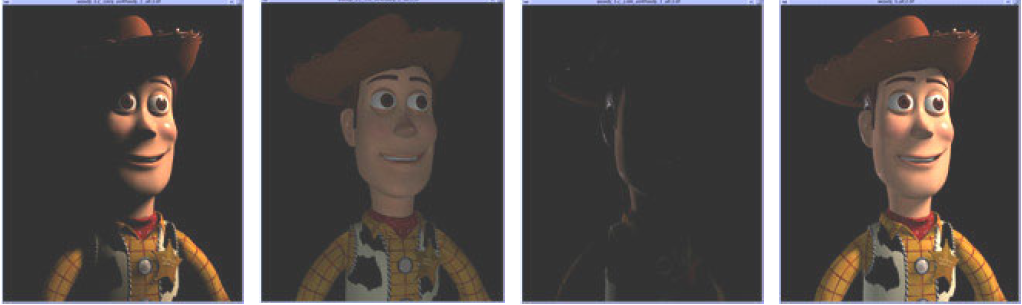
\includegraphics[width=0.7\textwidth]{Bilder/pixar keyrimfill.PNG}
	\caption{The use of Key, Fill and Rim Lights on Toy Story 2 \cite{sudeep}}
	\label{fig:woody}
\end{figure}

Often, in addition to the lights already mentioned, other sources of illumination are used to integrate the scene and its subjects. One of these is the "kicker light". It is usually placed on the opposite side of the key light and illuminates the corners of the subject that are not already covered by the key light. The main benefit of this type of lighting is to make the character or subject appear more three-dimensional. \\\\
Another light source often used is the "bounce light". These lights simulate reflections on subjects coming from other objects or another light source. Often these reflections are created by the real-time engine anyway, but the character and atmosphere of a scene can be adjusted separately. This can also suggest a more diverse scene to the player as is actually the case. \\
The following example (See Figure \ref{fig:teapot}) shows an example of how a virtual scene could be illuminated. It should be noted that this example is based on a static scene. Nevertheless, this lighting model is also possible for dynamic scenes, but the subject should then not be in the direct vicinity of the player, otherwise, there will be large changes in lighting \cite{Niedenthal1404353}. 
\begin{figure}[H]
	\centering
		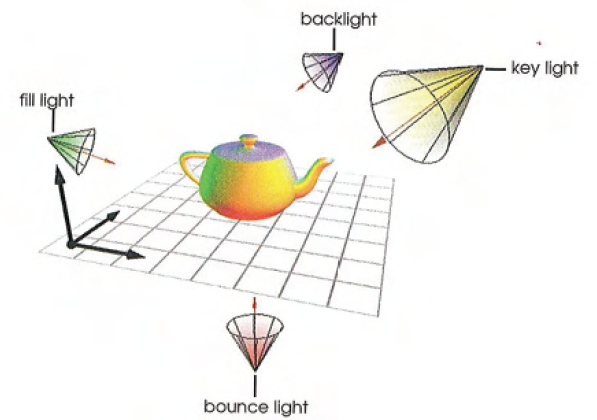
\includegraphics[width=0.7\textwidth]{Bilder/teapot.PNG}
	\caption{How a virtual scene may be lit \cite{Niedenthal1404353}}
	\label{fig:teapot}
\end{figure}
\newpage
In addition to the pure positioning of the lights, a number of other parameters of a light source can of course be set. The most obvious of these parameters are those that we already know from the real world, such as the color of the light, the brightness or the specularity. \\
The direction in which the light radiates can also be adjusted and parameterized by selecting the artificial light bodies. Possible are parallel, point, area and spotlights \cite{Shadowplay}. By carefully combining these, you can bring a scene to life and convey its atmosphere.\\
Even the form of light can, in case of area or spot light, be manipulated (see Figure \ref{fig:cookie}. This is done by using cookie textures, which act like a mask for the light source. This means that even complex patterns can be realized relatively easily in a virtual scene.
\begin{figure}[H]
	\centering
		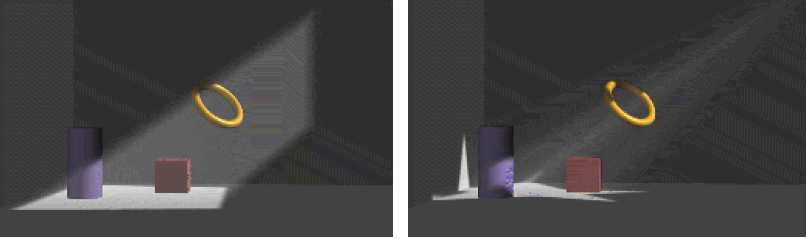
\includegraphics[width=0.7\textwidth]{Bilder/cookie.PNG}
	\caption{Using a cookie texture to modulate the appearance of a spotlight \cite{sudeep}}
	\label{fig:cookie}
\end{figure}

An additional immense advantage we have in virtual scenes is that virtual lights physically do not exist. This means that, unlike real films and their scene construction, we can place light sources anywhere in the scene. Another example for this is, that virtual lights can be programmed to have no fallof or to generate no shadows \cite{framework}\cite{sudeep}.

\section{Visual Styles}
\label{cap:highLow}
From the above methods, a quasi-infinite combination of illuminations can now be derived. For this reason, some categories were created to represent different styles \cite{Niedenthal1404353}. Lighting styles are described in terms of their tonal range, that is, the range of values from the darkest to the brightest light and the gray values in between. Lighting styles are also described in terms of the overall color, motivation, placement, and quality of highlights and shadows. \\

The character and mood of an image are significantly influenced by the tonal range from light to dark and by its distribution within the image. Those design decisions are decided early in the design process of a game or film. These decisions are usually motivated by the desired dramaturgy of the story and can be consistent throughout the time span of a scene or vary depending on the location and time of day or actions the player made on a given scene \cite{Niedenthal1404353}. While most of the categories and terms used to describe the lighting of a scene come from film and photography, many can be directly applied to the design of virtual scenes in video games. Two of these categories, which have a strong impact on the atmosphere of a scene, are high and low key lighting. These will be explained in more detail in the following paragraphs. 

\subsection{High-Key Stlye}
A light-hearted or comedic story might require a high-key lighting style. High-key lighting is a light setup for a scene that is predominantly well-lit with lots of soft fill light and mostly no harsh or shadows. The backgrounds, characters and set pieces also tend to be bright in color. That doesn't mean there are no dark areas, but the overall brightness tends to be light, the contrast is low, and the dark areas are soft and discreet. The result minimizes tension, as little is left to the imagination of the viewer or player\cite{Niedenthal1404353}. Which, in most cases, generates a light and relaxed atmosphere \cite{Storytelling}.

\subsection{Low-Key Style}
At the other end of the spectrum is low-key lighting. In a low-key lighting setting, most of the scene is darkly lit, with emphasis on the few areas that are brightly lit. The backdrops and costumes are usually darkly colored as well. The scene has a dark but not murky appearance. What is seen is as important as that which is not seen. The detail that is only hinted at is much richer than it would be with good lighting, this leaving a great deal of imagination left for the viewer or player and thus creating a more suspicious atmosphere \cite{Niedenthal1404353}. Light is used to direct the viewer's attention, darkness to stimulate his imagination \cite{Storytelling}.

\begin{figure}[H]
	\centering
		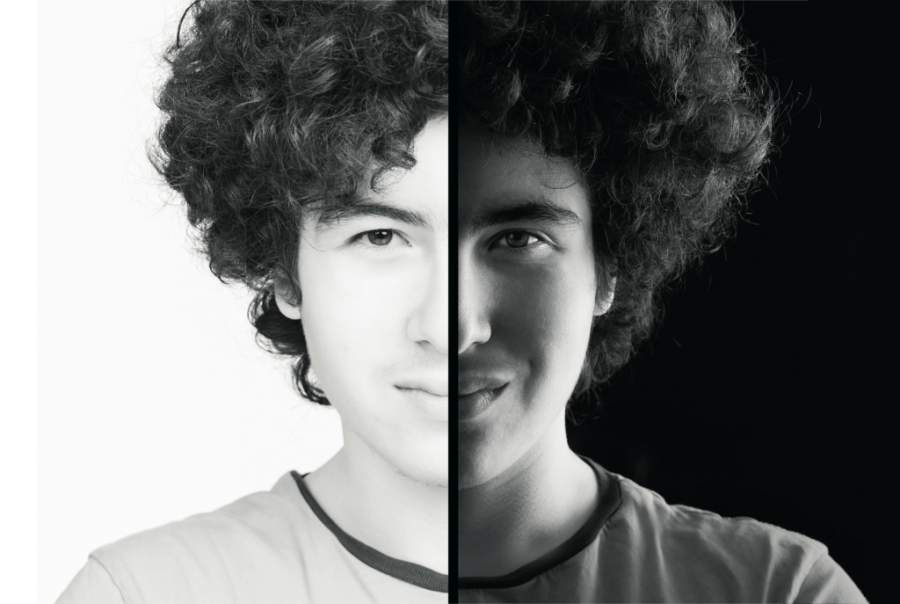
\includegraphics[width=0.7\textwidth]{Bilder/LowHighKey.jpg}
	\caption{High-Key (left) and Low-Key (right) lighting \cite{heisse}}
	\label{fig:cookie}
\end{figure}

Even before the viewer has understood the storyline, the lighting style can convey a feeling of a scene, especially when compared to scenes adjacent to it.Or within a single shot, one character can be modeled in light tones and another modeled in shadows and dark tones to suggest their individual personalities or their emotional or dramatic situations. This gives the viewer a first impression of the scene, which greatly affects the atmosphere and his feeling towards it\cite{Storytelling}.

\section{Creating Atmosphere through visual storytelling}
We can now examine how lighting develops and reinforces a story. As mentioned in the last chapter, the role of lighting can be roughly divided into the following  points \cite{sudeep} \cite{Storytelling}:

\begin{itemize}
    \item Directing the viewer’s attention
    \item Establishing a mood and atmosphere
    \item Creating a sense of depth
    \item Maintaining visual continuity
\end{itemize}

The main goal of lighting is to \textbf{guide the viewer's attention}. Lighting can be used to organize and prioritize elements and areas as well as characters in a scene. As Sudeep Rangaswamy has pointed out, effective lighting can divide a confusing scene with many distractions into individual, easy-to-understand areas \cite{sudeep}. Often the already established "three-point lighting" technique is used: A character is set off from his surroundings and background, which draws the viewer's attention strongly to him (see Figure \ref{fig:hopper}) \cite{Storytelling}. 

\begin{figure}[H]
	\centering
		
\includegraphics[width=0.7\textwidth]{Bilder/hopper.PNG}
	\caption{The contrast in lighting emphasizes Hopper from "A Bug's Life" \cite{bugslife}}
	\label{fig:hopper}
\end{figure}

Note the strong key light, which illuminates the character from above and leaves some areas of his face in shadow. In addition, the character has a strong rim light, which makes him stand out against the background. All other areas in the scene are more weakly lit. Even if the background now contains many elements, there is a strong focus on the character in focus.\\

Another visual effect to control the player's attention is playing with size differences and their weighting \cite{sudeep}. The following scene (see Figure \ref{fig:klee}) from the Pixar movie "A bugs life" will serve as an example: An ant standing on a cloverleaf is shown. The perspective in which the camera is placed and the shadow of the ant gives the viewer the feeling of being very small. 

\begin{figure}[H]
	\centering
		
\includegraphics[width=0.7\textwidth]{Bilder/klee.PNG}
	\caption{Scale and its balance help convey a bug’s view of the world. \cite{bugslife}}
	\label{fig:klee}
\end{figure}

This helps the viewer to adjust to his surroundings and creates a unique atmosphere of being very tiny \cite{sudeep}. Also, the rim light is used here to clearly set the cloverleaf apart from the sky, which is its background. Here, the sun shines directly on the cloverleaf (illuminating it from above), which makes it stand out strongly from the rest of the scene and the sky. This brings it very much into the foreground. In this example, the sunlight is the light that makes the sides of the clover shine, thus being both key and rim light \cite{sudeep}.\\

Another goal of visual effects and especially lighting is to give a mood and atmosphere to a given scene. This can happen mainly through the use of color: Very often, for example, red lights are used to excite the viewer and leave him with an uneasy feeling \cite{Shadowplay}. Calm, peaceful, scenes, on the other hand, are often lit with high key style. The scene is flooded with soft lights, there are few shadows that could hide details of characters and colors are used that are associated with peace and tranquility \cite{sudeep} (See Figure \ref{fig:flickvshopper} and \ref{fig:friedlich}).

\begin{figure}[H]
	\centering
		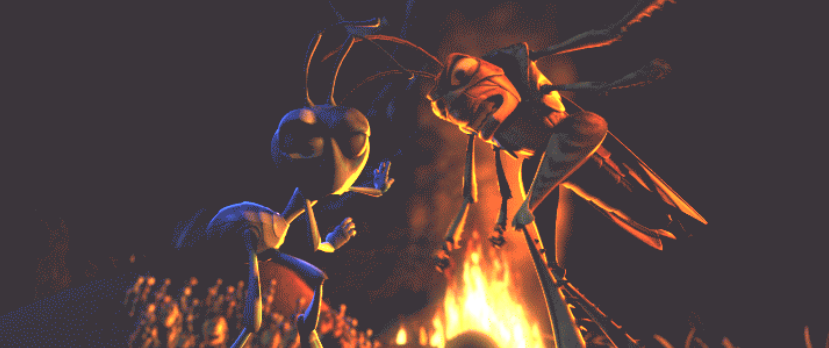
\includegraphics[width=0.7\textwidth]{Bilder/flickvshopper.PNG}
	\caption{A fight scene which is lit in low key \cite{bugslife}}
	\label{fig:flickvshopper}
\end{figure}

\begin{figure}[H]
	\centering
		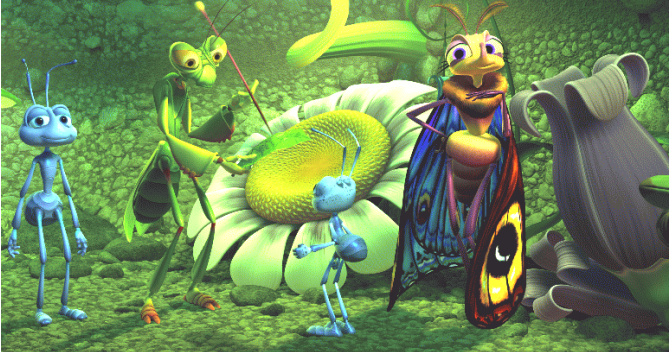
\includegraphics[width=0.7\textwidth]{Bilder/friedlich.PNG}
	\caption{A peaceful scene which is illuminated using high key techniques \cite{bugslife}}
	\label{fig:friedlich}
\end{figure}

Finally, another technique can be used to create a desired atmosphere: The use of shadows. Hard and distant light sources create crisp shadows. These produce a cold, sterile scene, giving the viewer or player an uncomfortable feeling. The shadows in Figure \ref{fig:sleeping} help evoke a dark, lonely atmosphere. Here, the glow of the television is the primary source of light, and the sleeping character casts an striking shadow on his couch. This arrangement of shadows, white lights and also the choosen perceptive arouses a lonely mood \cite{sudeep}. 
Notice how in this scene the character misses an rim light. This lets the character visually sink into his couch. 
\begin{figure}[H]
	\centering
		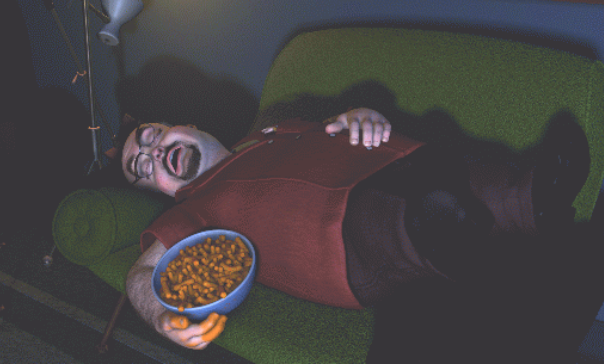
\includegraphics[width=0.7\textwidth]{Bilder/sleeping.PNG}
	\caption{Light from the TV casting shadows on a sleeping character from "Toy Story" \cite{toystory}}
	\label{fig:sleeping}
\end{figure}



On the other end of the spectrum, soft lights are used in warm and pleasing scenes because they create faint, barely noticeable  shadows \cite{Shadowplay} \cite{sudeep}.